\subsection{\textsc{SubBytes} transformation}
\label{sec:SubBytes}

The Byte Substitution layer can be viewed as a row of 16 parallel S-Boxes, each with 8 input and output bits (see Figure \ref{fig:aes-round-function}). 
Each state byte $A_i$ is replaced, i.e. substituted, by another byte $B_i$.

\begin{figure}[!ht] 
    \centering
    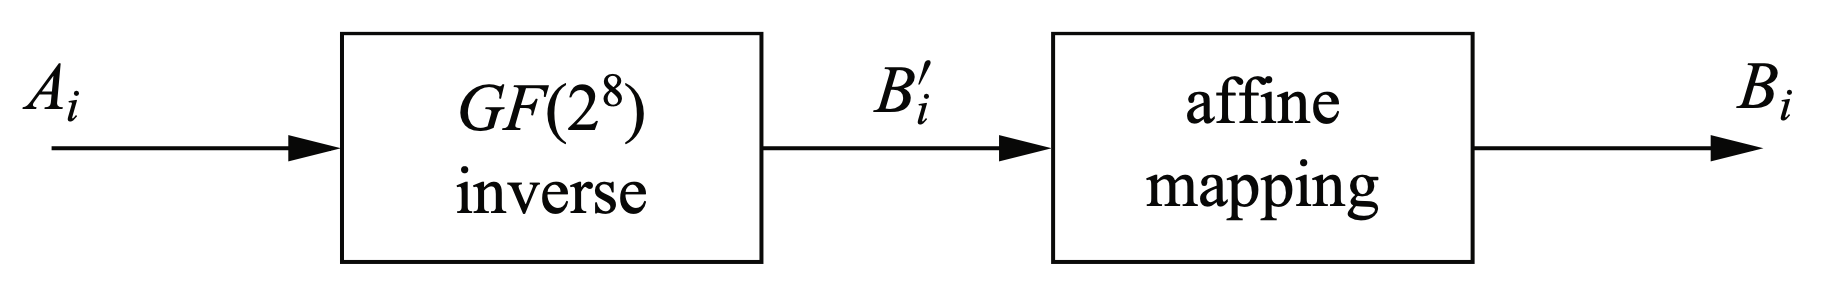
\includegraphics[width=.6\textwidth]{byte-substitution.png} 
    \caption{
        The two operations within the AES S-Box which computes the function $B_i = S(A_i)$ \cite{Paar2024}.
    }
    \label{fig:byte-substitution} 
\end{figure}

The \textsc{SubBytes} transformation is a non-linear byte substitution that operates independently on each byte of the state byte.
The S-Box is constructed by composing of two transformation:
\begin{enumerate}
    \item \textbf{Galois Field Inversion}: 
    Take the multiplicative inverse in the finite field $GF(2^8)$ and solve for ${B'}_i$ (Equation \ref{eq:gfi}), described in Section \ref{sec:multiplication}. 
    The element $\{00\}$ is mapped to itself.
    
    \begin{align}
        A_i \cdot {B'}_i &= 1 \mod P(x)
        \label{eq:gfi}
    \end{align}

    \item \textbf{Affine Mapping}:
    
    The following affine transformation (over $GF(2)$) is applied:
    \begin{align}
        b_i = {b'}_i \oplus {b'}_{(i+4 \mod 8)} \oplus {b'}_{(i+5 \mod 8)} \oplus {b'}_{(i+6 \mod 8)} \oplus {b'}_{(i+7 \mod 8)} \oplus c_i
    \end{align}
    for $0 \leq i \leq 8$, where $b_i$ is the $i$-th bit of the byte and $c_i$ is the $i$-th bit of a byte $c$ that is to be transformed.

    % Apply the following transformation with
    % each byte ${B'}_i$ is multiplied by a constant bit-matrix, followed by the addition of a constant 8-bit vector:
    % \begin{align}
    %     \begin{pmatrix}
    %         1 & 0 & 0 & 0 & 1 & 1 & 1 & 1\\
    %         1 & 1 & 0 & 0 & 0 & 1 & 1 & 1\\
    %         1 & 1 & 1 & 0 & 0 & 0 & 1 & 1\\
    %         1 & 1 & 1 & 1 & 0 & 0 & 0 & 1\\
    %         1 & 1 & 1 & 1 & 1 & 0 & 0 & 0\\
    %         0 & 1 & 1 & 1 & 1 & 1 & 0 & 0\\
    %         0 & 0 & 1 & 1 & 1 & 1 & 1 & 0\\
    %         0 & 0 & 0 & 1 & 1 & 1 & 1 & 1
    %     \end{pmatrix}
    %     \begin{pmatrix}
    %         {b'}_0\\
    %         {b'}_1\\
    %         {b'}_2\\
    %         {b'}_3\\
    %         {b'}_4\\
    %         {b'}_5\\
    %         {b'}_6\\
    %         {b'}_7
    %     \end{pmatrix}
    %     +
    %     \begin{pmatrix}
    %         1\\
    %         1\\
    %         0\\
    %         0\\
    %         0\\
    %         1\\
    %         1\\
    %         0
    %     \end{pmatrix}
    %     &\equiv
    %     \begin{pmatrix}
    %         b_0\\
    %         b_1\\
    %         b_2\\
    %         b_3\\
    %         b_4\\
    %         b_5\\
    %         b_6\\
    %         b_7
    %     \end{pmatrix}
    % \end{align}
    % where ${B'_i} = \left( {b'}_0, \dots, {b'}_7 \right)$ and $B_i = \left( b_0, \dots, b_7 \right)$
\end{enumerate}

% A lookup table for the \textsc{SubBytes} transformation can be generated by computing the substitution values for all possible two-digit hexadecimal inputs (i.e., 256 values from \texttt{00} to \texttt{FF}).
\textcolor{red}{insert lookup table}